%============================================================ 2. 관련 연구 (15쪽판)
%  국방발표 판의 3개 소절을 소제목 없는 세 문단으로 합쳤다. 문헌은 논지에 직접 쓰이는 것만 남겼다.
\section{관련 연구}
\label{sec:related}

방어 자산을 표적에 배분하는 문제는 주로 무기-표적 할당(WTA)으로 정식화되어 왔다~\citep{ahuja2007wta}.
그러나 실제 배정은 앞선 결정으로 어느 경로가 이미 막혔는지, 자산이 얼마나 남았는지에 따라
달라지므로, 고정된 거리·각도 비용만으로는 이를 표현하기 어렵다. 이에 본 연구는 배정 계층에 조합
최적화 대신 언어모델의 판단을 둔다. 무인 위협을 무력화하는 수단 가운데 연성 대응은 유선으로
조종되는 표적에 통하지 않고, 경성 대응은 값싼 표적에도 고비용의 자원을 써야 하는 부담이 있다.
이러한 한계 때문에 본 연구는 저비용의 그물을 이용한 물리적 포획을
택한다~\citep{wang2021cuas, sutea2026fiber, rumbaugh2024cost}. 해상에서 강화학습으로 표적을
포위하는 기존 연구~\citep{zhang2025encircle}는 방어정이 표적보다 빠르거나 비슷한 속도라고
가정한다. 그러나 실제 방어정은 고속으로 돌진하는 자폭 USV보다 느린 경우가 많기 때문에 본
연구에서는 방어정이 표적보다 느린 조건에서도 방어할 수 있도록, 표적의 경로에 먼저 가서 그물로
막는 선제 차단 방식을 제안한다.

기존 다중 에이전트 강화학습은 주로 중앙에서 학습하고 각자 실행하는 구조를 따르며, 팀 보상에서
개체별 기여를 분리하기 위해 가치망 학습에 의존한다~\citep{rashid2018qmix, foerster2018coma, yu2022mappo}.
그룹 상대 정책 최적화(GRPO)~\citep{shao2024deepseekmath}는 같은 상태에서 뽑은 여러 후보의 보상을
서로 비교해 가치망 자체를 없앤다. 본 연구는 GRPO를 다중 에이전트 제어로 확장하여, 후보 하나는
기하 휴리스틱으로 고정해 기준선으로 삼고 각 후보의 팀 보상은 시뮬레이터를 다시 진행해 얻는다.
이로써 정책은 부정확한 가치 추정에 흔들리지 않고, 휴리스틱보다 나은 행동을 후보 행동 간 직접
비교로 찾아가며 학습한다.

\begin{figure*}[!t]
\centering
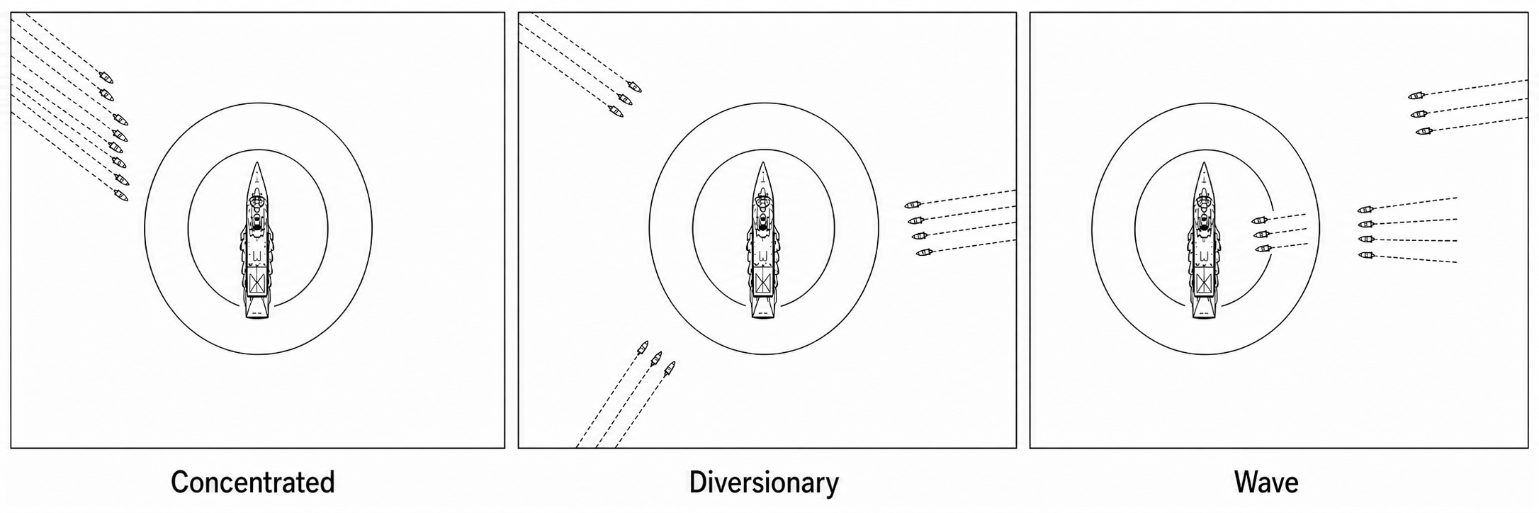
\includegraphics[width=\textwidth]{fig2.png}
\caption{세 가지 공격 포메이션: 집중·양동·파상(좌$\to$우)}
\label{fig:formations}
\end{figure*}

U-Net~\citep{ronneberger2015unet}처럼 영상의 픽셀마다 값을 매기는 신경망과, 여기에 영상 전체의
정보를 덧입히는 조건 변조 기법~\citep{perez2018film}은 주로 영상 속 영역을 구분하는 데 쓰였다.
한편 Pointer Network~\citep{vinyals2015pointer}나 어텐션~\citep{vaswani2017attention}처럼 여러
후보에 점수를 매겨 하나를 고르는 출력은 주로 조합 최적화에 쓰였다. 본 연구는 두 방식을 결합하여
픽셀마다 매긴 점수, 즉 점수맵을 이동할 지점의 선택 확률로 삼는다(\ref{sec:policy}절). 따라서
행동이 지도 위의 한 지점이 되어 공간 구조가 보존된다. 또한 특정 격자를 미리 선택 후보에서
배제하는 방식으로 안전 제약을 지키며, USV 정보를 지도 위 격자에 담으므로 USV 수와 무관하게 입력
차원이 고정되어, 그 수가 달라져도 유연하게 대응할 수 있다.

언어모델에게 계획을 맡기는 기존 연구는 지시를 실행 가능한 단계로 나누고 실행할 수 없는 계획을
차단하며~\citep{huang2022zeroshot, ahn2022saycan}, 출력을 정해진 형식으로 받아 기존 시스템이 읽을
수 있게 한다~\citep{openai2026function}. 언어모델은 전장 상태와 임무 목표, 교전 규칙 등을 함께
읽으므로 비용 함수를 재설계하지 않고도 배정 기준을 유동적으로 바꿀 수 있다. 본 연구는
언어모델에게 배정만을 맡기고, 기동 계층에서는 격자 단위로 판단하는 모델과의 결합으로 언어모델이
배정에만 집중하고 그 출력이 불확실하더라도 위험한 기동으로는 이어지지 않게 한다(\ref{sec:validmask}절).
